\documentclass[11pt,letterpaper]{article}

\usepackage{graphicx}
\usepackage[margin=1in]{geometry}
\usepackage{amsmath}
\usepackage[T1]{fontenc}
\usepackage[utf8]{inputenc}
\usepackage{authblk}
\usepackage[titletoc,toc,title]{appendix}
\usepackage{fancyhdr}
\usepackage{lastpage}
\usepackage{listings}
\usepackage[parfill]{parskip}

\pagestyle{fancyplain}
\fancyhf{}
\fancyfoot[R]{\footnotesize Page \thepage\ of \pageref{LastPage}}

\renewcommand{\headrulewidth}{0.0pt} % No header rule
\renewcommand{\footrulewidth}{0.4pt} % Thin footer rule

\begin{document}

\title{Graph-Based Analysis of Relational Data:\\ An Intermediate Progress Report}

\author[ ]{Konstantinos Xirogiannopoulos}
\author[ ]{Benjamin Bengfort}
\affil[ ]{Department of Computer Science}
\affil[ ]{University of Maryland}
\affil[ ]{\textit{\{kostasx,bengfort\}@cs.umd.edu}}

\date{April 10, 2015}

\maketitle

% Introduction %

\section*{Introduction}

Graph-based analyses have become increasingly popular in recent years, particularly for large scale machine learning upon sparsely connected, highly related data sets. Graph data structures have become invaluable to large scale search, aggregation, and transformation tasks on connected data sets by allowing groups of nodes to be operated on via edge traversal, minimizing the amount of processing required from the point of view of the initial set of vertices \cite{berretti_efficient_2001}. The popularity of these techniques, combined with the growing sense that graphs model the real world effectively, have led to the development of parallel, large scale graph computation  engines and more recently, native graph databases.

% In the real paper we should probably get to the point a tad quicker.

There are many motivations for utilizing graph algorithms in coordination with a variety of data stores with different physical and logical organization. Firstly, graph traversals and computations can be more easily expressed in a graph-specific query language like Gremlin \cite{rodriguez_gremlin_2013} or Cypher \cite{miller_graph_2013} rather than a declarative or low level programming language \cite{rodriguez_exploring_2012}. Lightweight expressions of graph operations lend themselves very well to efficient, lightweight implementations of machine learning algorithms and provide inherent efficiency. When data can be easily modeled as a network or through connections (and more and more data is seen this way thanks to social networks, genomic research, entity resolution and more), the index free adjacency and other properties of graphs allow efficient computation of shortest paths, centrality, community detection, and more. In fact, the idea of vertex-centric computation \cite{malewicz_pregel:_2010} means that graph algorithms scale well and can be leveraged not only in transactional data systems, but also in distributed computation.

Although there is utility in the implementation of graph algorithms there are also many tensions that are expressed by the wide array of current research on the topic. First - graph algorithms can be computed locally for a small group of nodes in a transactional fashion \cite{jadhav_comparative_2014}, or at scale across extremely large networks for population-wide analyses \cite{cuzzocrea_big_2014}. In both cases, the base data set is usually too large to fit into memory, requiring some form of data storage and management. This has led to two primary trends: the development of native graph databases that leverage ideas from the NoSQL movement and the development of large scale, parallel online analytical (OLAP) graph processing.

However, relational databases have been well studied and optimized in their longer history. RDBMS systems are extremely performant as transactional systems where few records are selected, inserted or updated at transaction time. Although this model doesn't lend itself to larger scale analytics, RDBMS systems play vital operational and theoretical roles in the larger database space. Many studies have concluded that relational databases, while not specifically designed for graphs, are still tools that can be extended to provide solutions for graph-based algorithms \cite{welc_graph_2013}, \cite{najork_hammers_2012}, and \cite{vicknair_comparison_2010}.

% Nice paragraph below!

In this paper, we outline the ongoing progress towards creating a system for efficient in-memory graph analytics using relational data. Our ongoing work has mainly focused on defining some initial specifications of our declarative Datalog-based DSL, and various optimizations. The optimizations that we have implemented facilitate a more efficient extraction of the graph from the relational schema -- both in terms of time complexity and memory usage. For our implementation, we used Java and the popular BluePrints library to expose an API familiar to many users. Our main paths of progress to date include the following:\\

\begin{enumerate}

	\item Defining initial specifications for our declarative DSL, and writing a parser and translator to SQL.
	\item Expanding the functionality of the DSL towards and optimizing extraction for ego-networks.
	\item Minimizing the memory footprint of the extracted graph via a \textit{compressed representation} %compressed Report

\end{enumerate}

% In this survey we take a close look at the use of databases for graph analytics, from graph structured database management systems that are designed to support transactions to large scale parallel graph processing that occurs offline and asynchronously. We will then move forward to review how relational databases have been affected by or utilized in graph computing and discuss a variety of computational models that are related to our research proposal, \textit{Graph-Based Analysis of Relational Data}. Finally we will conclude with a slightly deeper look at ongoing research of applications that are related to our proposal, namely Grail \cite{fan_case_2015}, Vertexica \cite{jindal_vertexica:_2014}, and Trinity \cite{shao_trinity:_2013}.

% \section*{Non-Relational Graph Computing}
%
% In this section we start by exploring systems that are \textit{specialized} for graph computation and processing. Particularly we explore NoSQL solutions and native graph databases, as well as approaches for distributed graph computation and OLAP graph analyses. Finally we will present critiques of non-relational techniques from the relational perspective.

% \subsection*{NoSQL Solution: Native Graph Databases}
%
% \begin{figure}
% 	\centering
%     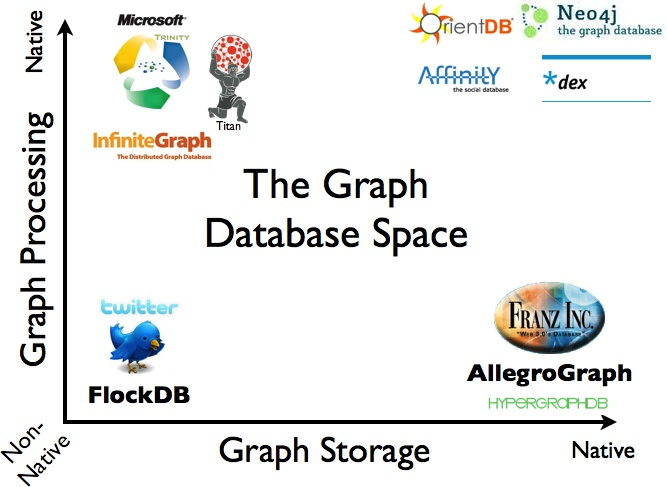
\includegraphics[width=0.80\textwidth]{figures/graphdb_space.jpg}
%     \caption{\textsf{The graph database space is characterized by native graph processing and native graph storage, popularized by this graphic originally published in \cite{robinson_graph_2013}. A third, not shown dimension of the graph database space is parallel or distributed graph computation engines.}}
%     \label{fig:graphdb_space}
% \end{figure}
%
% Although we are a long way from the CODASYL vs Relational “Great Debate” in the early 1970s \cite{stonebraker_what_2005}, it seems that we may be seeing network/hierarchical models coming back around to compete with relational databases, now re-branded as Graph Databases and NoSQL or NewSQL. This is especially apparent when you consider the popular categorization of graph database systems by native or non-native graph processing and graph storage as shown in Figure \ref{fig:graphdb_space}, originally published in \cite{robinson_graph_2013}. Looked at from the point of view of the “Great Debate”, these axes represent logical and physical dependencies of  a graph-specific database.
%
% At the completely non-native end of the scale, FlockDB \cite{kallen_flockdb_2012} uses text-based data storage of adjacency lists to perform fast and scalable transaction-like operations on graphs particularly for high throughput applications like web sites. Flock was particularly used at Twitter as a fast query, sharded, in-memory processor of relationships. On the other end of the scale, there is OrientDB \cite{_orientdb_2015} and Neo4j \cite{eifrem_neo4j_2014} that are complete database management systems and that store vertices and edges of graphs on disk in a physical layout specifically optimized for vertex-centric computation and traversal. These systems also provide built in graph processing, which developers express through a query language - OrientSQL and Cypher respectively.
%
% Titan \cite{broecheler_titan_2015} takes a different approach, allowing the user to choose native storage of either BerkelyDB, Cassandra, or Apache HBase. Titan provides native graph processing through the Gremlin query language, which is directly translated to the back-end data store using Tinkerpop. Titan also has a distributed graph computation engine called Faunus. Finally, HypergraphDB \cite{iordanov_hypergraphdb_2012} provides native graph storage and can be used as an embedded data storage layer in other applications that have internal graph processing requirements. Similarly, at Facebook, TAO \cite{bronson_tao:_2013} is a distributed data model, which provides efficient read-optimized access to their internal data model - the social graph.
%
% This brief survey of graph databases shows that the primary mechanism that commercial solutions have used to improve graph oriented performance is through the use of columnar or key-value storage. Even solutions like Titan that have no associated storage layer prefer columnar storage like HBase or Cassandra. It is important to note that most of these data stores do not provide full ACID guarantees (although OrientDB and Titan with BerkelyDB attempt to provide a limited subset of the ACID guarantees) and prefer block-at-a-time processing, especially when those blocks are most likely going to be neighborhoods of the vertex being processed (or a root block). Our research must show that a relational database solution not only is able to perform equivalently to a native graph database solution, but that there are often advantages to using a relational model of processing in graph algorithms.

% \subsection*{Large Scale, OLAP Graph Processing}
%
% An advantage of graph algorithms is that they provide efficient means of computation over large data sets by traditionally focusing on locality (vertex neighborhood within a particular number of hops), index-free adjacency, and message passing. This has made graphs ideal for use in a MapReduce or distributed computation context, and in fact graph processing for large data was a significant part of the advent of Big Data at Google via PageRank \cite{page_pagerank_1999}. As such a number of graph computation frameworks ignore the data management portion and instead rely on transformations and preprocessing to load and compute on a graph in an OLAP, distributed fashion.
%
% Of these systems Pregel \cite{malewicz_pregel:_2010} and its open source counterpart,  Giraph \cite{ching_apache_2014}, have perhaps had the most impact on distributed graph computing utilizing existing cluster resources. The primary method of computation is iterative - bulk synchronous updates. This contrasts to a growing framework particularly implemented for machine learning - GraphLab \cite{low_graphlab:_2011}, which implements a gather, analyze, sort (GAS) model of computation for iterative machine learning.
%
% Newer approaches include GPS \cite{salihoglu_gps:_2013}, which uses a similar computational model to Pregel, but optimizes the API to be more expressive of common graph tasks as well as the distribution (partitioning) of vertices to improve performance especially for high-degree nodes. The most recent library, GraphX \cite{_graphx_2015} utilizes an in-memory computation framework, distributing vertices and edges for processing across resilient distributed datasets (RDDs).
%
% A prototypical workflow for graph computation utilizing distributed OLAP graph processing upon a large data store (in this case a relational one) is as follows:
%
% \begin{enumerate}
% 	\item Use Sqoop or a database dump to export data to HDFS or HBase
% 	\item Perform MapReduce preprocessing, formatting data as edges and vertices
% 	\item Run computation using Giraph, GraphX, etc.
% 	\item Perform MapReduce postprocessing to transform data back to schema
% 	\item Use Sqoop or database import to load back into a relational store.
% \end{enumerate}
%
% Clearly, when considering this workflow, reduction in the scope of processing is vital as error, complexity, and time is injected at every phase of this workflow. Some online data store is required, and a relational database is a good choice. In order to further explore the use of relational data stores for computation, we should consider both transactional and local graph computation as well as whole-database OLAP computations. Parallelizing computation, especially using an in-memory, iterative framework will be extremely important to show how many types of pattern-matching and ML algorithms can be implemented leveraging relational resources like indices and lookup tables.

\section*{Datalog as a facilitating language to SQL}

The primary critique for using relational databases in graph computation is that the primary programming abstraction, SQL, is declarative and not well suited to the description of graph algorithms. Graph-specific query languages like Gremlin \cite{rodriguez_gremlin_2013}, Cypher \cite{miller_graph_2013}, and SPARQL \cite{prudhommeaux_sparql_2008} are able to easily express traversals and computations required for graph algorithms. Because these DSLs are directly related to the graph computational model, their expressive power and execution context are fundamentally different than that of the traditional iterator-model of relational databases. For example, Gremlin exposes a pipeline-iterative mechanism of computation and SPARQL can be directly translated into lambda calculus.

As a result, there has been interest in the use of Datalog, a declarative programming language, to extend relational algebra into the graph algebra domain \cite{he_graphs-at--time:_2008}. When graph computations can be expressed as a query operation selection operators can be generalized to pattern matching and composition operators can be included to rewrite graphs. Because Datalog is a syntactic subset of Prolog, it can also be used as a query language for deductive databases. Recent advances have adapted Datalog with recursion and extended Datalog specifically for graphs \cite{shkapsky_graph_2013}, \cite{green_datalog_2013}, allowing for aggregation, negation, and typing - monotonic constraints that are fundamentally a part of a relational database.

The conversion of Datalog queries to SQL queries, thereby extending relational processing with graph aware processing is not just isolated to recursion on a single machine, but has also been shown to be parallelizable \cite{seo_distributed_2013}. Datalog has also been shown to be easily extensible to large scale machine learning on big data sets \cite{bu_scaling_2012}.

Datalog is clearly a fascinating choice for research as it has been shown to be complete and effective at graph computation, usable on a relational database, and parallelizable. Previous work has focused on the adaption to new graph domains, but there has been no complete system where Datalog augments a relational database in a specific fashion for both parallel and efficient graph computation.

% \subsection*{Conversion of Relational to Graph}
%
% An alternate idea to the querying of data stored in a relational database via a query language that expresses graph computation is to simply export a part or whole of the relational database to disk or to memory where it can be operated upon using the graph specialized techniques. This is especially important in domains like RDF where neither the physical nor the logical layer of the database is well suited to the data model of the graph \cite{hert_comparison_2011}. Export techniques focus on the abstraction of the relational model, its conversion, or efficient, large scale ETL techniques.
%
% In \cite{de_virgilio_converting_2013}, De Virgilio et al. explore the direct conversion of a relational data store to a property graph model. Their model exploits the schema of the relational database as well as its constraints in order to translate conjunctive SQL queries into graph traversals. Because they target a complete conversion, full serialization of all tuples and expensive joins are required during the conversion process.
%
% Extract-Transform-Load tasks are essential database management operations, especially if they can reduce three or more steps proposed in the prototypical workflow of distributed or OLAP graph computation. GraphBuilder is a system used to offload the complexity of graph construction, formulation, and serialization both into and out of relational data stores during offline processing \cite{jain_graphbuilder:_2013}. GraphBuilder enables the use of scalable analytics using a distributed framework like MapReduce and eases some of the complexity in the workflow described earlier, having significant performance impacts.
%
% De Virgilio et al. are the first of these readings to describe the scenario where a relational database might be introspected to produce a property graph model with little definitional requirements from the user or the target. GraphBuilder shows a path to operationalizing parallel graph computations with a reduced work load. In both cases, processing is handed off to another graph system, but the possibility of a single system that operates similarly fits in well with our proposal.

\subsection*{DSL Definition and Implementation}

\begin{figure}[t]
\centering
\scriptsize
\begin{lstlisting}[breaklines,basicstyle=\ttfamily]
(1) Nodes(ID, Name) :- Author(ID, Name)
    Edges(ID1, ID2) :- AuthorPub(ID1, PubID),
                       AuthorPub(ID2, PubID)
(2) For Author(X, _).
      Nodes(ID, Name) :- Author(X, Name).
      Nodes(ID, Name) :- AuthorPub(X,P), AuthorPub(ID,P),
                   Author(ID, Name)
      Edges(ID1, ID2) :- Nodes(ID1, _), Nodes(ID2, _),
                   AuthorPub(ID1, P), AuthorPub(ID2, P)
\end{lstlisting}
\vspace{-10pt}
\caption{Graph Extraction Query Examples}
\vspace{-10pt}
\label{fig:queries}
\end{figure}

A core piece in the implementation of our project is the correct and thorough implementation of a translation module which converts a graph-sepcific Datalog DSL to SQL, in order to perform relational operations. Although in the majority of cases, there is a very straightforward mapping of the two languages, no open source implementation of the translator was readily available. We were therefore required to write our own implementation.

The translation of Datalog to SQL centers around the process of mapping predicate symbols of \textit{atoms} (predicate symbols along with their list of arguments or terms) to database tables and terms to columns within those tables. The actual name of the term in the queries does not need to directly mirror the database; it can simply be an alias. The key idea behind mapping is that the ordering of arguments reflects the order of the columns in the database table. Each alias is therefore directly mapped to a projection of the column that appears in that position in the table. The left-side terms also must appear either in the right side, or somewhere else in the query as variables - an important technique that will be further discussed in the next sections. A balancing of terms is necessary to ensure the left side does not represent an existent predicate (table), but that the view will be generated using right-side predicates.

In our initial implementation, the translator was achieved using a \texttt{Lexer}, which parses the DSL using \textit{regular expressions}, returning an \texttt{iterable} of the individual tokens which make up the query. Each token is tagged with a specific label depending on its position in the query. For example, in query (1) of Figure \ref{fig:queries}, \texttt{Author} and \texttt{AuthorPub} are names of relations, so the arguments will be treated as the aliases of the adjacent columns in those exact positions in the underlying table. Because the user is assumed to have full access to and knowledge of the database's schema, we leave the left and right side balancing as a necessary user provided restriction.

\subsection*{Extending Datalog for Ego-Graphs}

In order to define an expressive DSL for graphs, we explored the types of operators that are necessary to expanding the relational domain in a meaningful way, such that operators are meaningful and intuitive. Our current approach is to extend Datalog to support an iterative \texttt{For} loop. This loop functionality facilitates the extraction of a specified \textit{set} of multiple graphs rather than a single graph. For example, $N$-hop \textit{ego-networks} are very interesting for a variety of tasks and analyses and can be extracted from multiple graphs. Given a single node (the ego), an $N$-hop ego network is the neighborhood of the ego, as well as the neighborhoods of the neighbors up to $N$ links away from the center. To extract this subgraph from multiple graphs, some form of recursion is required.

The \texttt{For} loop we have implemented is showcased in query (2) of Figure \ref{fig:queries}. In this query the loop iterates through every \texttt{Author.Id} (the \texttt{Id} is the first column) in the \texttt{Author} table, and computes the graph specified in the indented queries below, which includes all Authors who have published with author \texttt{X} in the nodes, as well as edges between those authors, defined the same way. This query will extract the 1-hop neighborhood for author \texttt{X}, and will repeat for each value of \texttt{X} in the database.

\subsection*{Optimizing the Extraction of Ego-Graphs}

Under normal execution, our system translates our Datalog DSL into standard SQL and executes the appropriate queries against PostgreSQL. Unfortunately, when using the \texttt{For} loop to specify more than one graph, this operation makes continuous queries to the database, receiving independent results -- a hugely expensive operation in terms of time and memory. For instance, if a user wanted to extract and apply analytics on the entire range of ego-graphs within a table, the amount of queries made against the database would equal the number of distinct IDs. We have found that there is substantial overhead associated with every distinct query to the database, whose effects become limiting even in small datasets.

In order to minimize computational time, we have attempted to reduce the amount of computation required by PostgreSQL, moving work to our software, thereby reducing the need for constant queries to the database. In particular, this tactic optimizes the extraction of an entire range of ego-graphs. We have developed a mechanism which requires only a single query to PostgreSQL in order extract all of the necessary information for creating all specified, in-memory graphs.

This mechanism uses a \texttt{union of queries} operation in order to fully use a single SQL query for obtaining all edges in the entire graph. This single large query contains any and all of edges required for obtaining ego-graphs, and is therefore sufficient without further calls to the data store. By using the result set from the Edges query as a view via a \texttt{WITH} query, we were able to apply a \textit{tag} to each tuple of the result set such that the aggregation of tags signfies an ego-graph in which the specific edge participates. An example of a query which is used to achieve a similar result is described in Figure \ref{fig:tagging}. This query returns a result set where each edge is tagged with the ego-graphs the vertices particpate in, and allows for the construction of 1-hop neighborhoods for each Node in the range of the query.

In order to construct the graphs after completing these steps, the only processing required is a single pass through that result-set. We then create each ego-graph, as we go along, adding edge after edge as we come across it, to the adjacent ego-graph that is specified in the aggregated array of tags for that edge. The performance gains in applying this optimizations appear to be substantial. For the aforementioned subset of the DBLP dataset, the total time to extract the neighborhoods of all nodes in the co-authors graph came down from 18s to approximately 2.2s using this optimization.

\begin{figure}[t]
\scriptsize
\begin{lstlisting}[breaklines,basicstyle=\ttfamily]
WITH Edges AS (<SQL Query for the Edges>),
Result AS
(
SELECT DISTINCT e1.X AS e1u, e1.id2 AS e1v, X as TAG
FROM Edges e1
WHERE e1.X IN (SELECT DISTINCT X FROM Edges)

UNION

SELECT DISTINCT e2.X, e2.id2,e1.X AS TAG
FROM Edges e1,Edges e2
WHERE e1.X IN (SELECT DISTINCT X FROM Edges) AND e1.id2=e2.X
)
SELECT e1u,e1v,array_agg(tag) FROM Result GROUP BY e1u,e1v;
\end{lstlisting}
\vspace{-10pt}
\caption{Result-Set Tagging for Efficient Ego-Graph Extraction}
\vspace{-10pt}
\label{fig:tagging}
\end{figure}


\subsection*{Compressing the Output Graph}

%resultset  can get large
After the queries in our DSL are translated to SQL applying the above optimizations when necessairy, the next step is to generate and load the graph into memory. The size of the result-set after the produced SQL is executed against the database, depends on two factors; (1) the current size of the participating tables in the database, and (2) the amout of predicates in the query that could potentially narrow down the size of the result-set returned. To eliminate  the latencies associated with moving data back and forth from disk to memory, the entire graph is required to reside in memory for the entirety of the computation. Another goal we aimed for was thus to decrease the memory footprint of the generated graphs by our system, in a lossless fashion that would continue to allow vertex centric programs to run against the graph.

%we did it with this high overview idea
The way we accomplished this is by using a \textit{compressed representation} of the graph. Methods like this one been studied in the past \cite{feder_1995}, and revolve around the idea of compressing the number of edges in highly condensed cliques, to a minimum, by having each of the nodes in the clique connect to only a single \textit{virtual} node instead.

%this is why we did it
In most cases, graphs are comprised of nodes of the same \textit{type}, being connected to each-other in various ways. In order to materialize these connections in the form of edges, a \textit{self join} is usually required. Self-joins are simply join operations where we are joining a table with itself, in order to find the intersections between two of its own columns, based on some predicate. When the size of the table starts getting reasonably large however, these self-joins become increasingly slow to complete, quickly reaching a point where the query is essentially impossible to run in a reasonable amount of time.

%this is how we did it
Our solution to this problem is that instead of pushing the self-join to PostgreSQL, we instead delay the self-join and apply it directly to the final graph. In essence, this means the actual join operation will only be computed gradually, and only when the computation requires a node to send a message to its neighbors. The implementation of this path is quite simple. With a single projection of the table that needs to be self-joined, and a sequential scan over it, we create a \textit{virtual} node for every distinct destination vertex, (where the destination vertex is the join condition for the self-join) and serially attatch nodes to their adjacent virtual nodes accordingly.

%this is what it gives us
Many large real-world graphs can contain a substantial amounts of very densely connected cliques, where many nodes are all connected to each-other via seperate, distinct edges. This representation will hence allow for substantial amounts of compression. As an example, going back to the aforementioned DBLP example dataset, for a publication with k authors, the co-authors graph contains $k(k-1)/2$ edges between those authors. By using the compressed representation, the number of edges per clique get compressed to the minimum of $k$ edges (just one for every one of the $k$ nodes), with the (usually) small trade-off of one extra node. The benefits of using such a representation of the graph are therefore two-fold; (1) by amortizing the latency of  self-joins, it allows for extracting larger graphs from very large relational tables, that were otherwise impossible to extract by actually computing the self-join, and (2) they naturally result in graphs with a significantly smaller memory footprint, thus enabling analytics on larger graphs. This representation is currenlty as a subclass on top of \texttt{TinkerGraph}, which entails many limitations which we intend to move away from in the future versions.

%Graph Processing on Relational Datastores

\subsection*{Related Work}

% Critique of Non-Relational methods
% The fact that the use of a distributed processing framework or graph native database for these efficient types of computations isn't necessarily a direct response to problems with a relational organization of data. Instead they can be seen as fulfilling of some other requirement - the use of distributed computation frameworks, or an optimization of vertex-by-vertex computation. However,
Since the advent of specialized systems, there has been some criticism from the relational community that a specific-framework isn't required. The primary line of thought is that relational databases can perform competitive or superior performance for most implementations and that the benefit of specialization is far outweighed by the cost of replacing an existing infrastructure \cite{welc_graph_2013}.

There is a fair amount of past and ongoing work on using relational datastores for graph computation. This work mostly focuses on doing so by means of SQL queries against the database. Most of these systems support and expand on the notion that there may be no real need for the existence of specialized graph computation frameworks, and attempt to prove this by means of creating these systems.

Grail \cite{fan_case_2015} is a syntactic layer for querying a graph in a vertex-centric way such that the graph is stored in an relational database management system
\cite{fan_case_2015}. The authors of Grail propose a query language that can then be translated into SQL and executed upon relational tables of vertices and edges. The authors hope to show that a relational datastore is both productive and performant in graph computations and that a specialized system is not necessary. They also lay the foundation for considering the construction of relational devices like indices and tables for graph-specific querying on existing data.

Vertexica \cite{jindal_vertexica:_2014} also provides a graph analysis toolkit on top of a relational database, similarly injecting data storage, query processing, and query interface support to the relational system for vertex-centric graph analysis \cite{jindal_vertexica:_2014}. Vertexica also uses a vertex/edge table for querying data, provides per-vertex transactions, and uses indices for fast retrieval of message passing. Vertexica also introduces many interesting graph-specific optimization techniques that are reminiscent of the columnar/relational database that the system sits on top of. In particular, they implement table unions to avoid expensive three way joins, parallel workers, batching, and late materialization.

Finally the Trinity \cite{shao_trinity:_2013} database, while not on a traditional relational store, implements a distributed graph engine on a memory cloud (a key-value store that is loaded into memory) for low latency graph queries \cite{shao_trinity:_2013}. Trinity, similar to Grail and Vertexica, implements a graph query layer called TSL that allows users to declare a schema and vertex-centric computation that is translated to the storage layer. Trinity's storage layer is strikingly similar to the aforementioned systems, and the distributed hash table (DHT) for vertices seems to be implemented primarily for distributed storage and fast access by the Trinity cluster. Potentially a sharded relational cluster would serve the same requirement.

It is therefore apparent that the main goals of this work are very different from the aforementioned systems. Our goal is to provide a layer of abstraction that will allow users to apply in-memorty graph analytics on their already existent relational data, without assuming that their data is already in graph format (tables of Vertices and Edges), in contrast to these related works.

\section*{Discussion}

Because specialized systems for parallel graph processing and native graph computation exist, any system that is researched or developed must be at least comparable to the specialized systems. Two considerations for the system are related to the non-relational techniques:

\begin{enumerate}
	\item ACID transactions on local subsets of vertices and edges
	\item Fast, parallel offline analyses of large portions of the database
\end{enumerate}

Specialized systems focus on storage layers that optimize their ability to lock vertices and their edges in a contiguous fashion without blocking other transactions. Parallel graph computation frameworks focus on two primary methods: vertex-centric computation and gather-analyze-sort (GAS) models. Relational databases have been researched extensively to provide both transaction isolation and serializability as well as parallel forms of computation, hopefully we can build upon that research to provide operation comparable to specialized systems.

It is clear that the programming interface to graph computations on a relational database must be graph specific, SQL is declarative but not expressive enough for most types of iterative or recursive computations. Datalog appears to be an extremely good candidate, as work has been done to ensure that Datalog is able to easily operate on graphs or be translated to a relational structure.

Conversion techniques on top of existing relational stores indicate that graphs may be induced or inferred from existing structures with user intervention. This seems to indicate there is no need for predefined vertex, edge, and message tables. However, these tables might be useful as non-persistent in-memory indices or data structures to optimize or improve computation.

Based on what we've learned from our previous survey \textit{A Survey of Graph Analyses using Databases}, our work has so far focused on the Flexible extraction of a graph from an existing data store into memory for computation (reducing the impact of join operations), and will continue by potentially exploring:

\begin{enumerate}
	\item Efficient implementation of the condensed representation, moving away from the TinkerGraph model.
	\item Use of existing relational tools (indices, stored procedures, operators) to improve graph processing in a meaningful way.
	\item Extensible graph inference and creation from the schema of a relational database and exposure to these graphs from a graph-specific query language.
\end{enumerate}

Therefore while our proposal has some similarities to the Datalog papers, the conversion papers, and the three systems that produce graph operators on top of relational operators - we intended to produce a complete system that is both fast and efficient for graph processing on top of existing, native relational storage.

\section*{Conclusion}

Graph analyses and computations are important for efficient and large scale machine learning and local queries and traversals. Since much data is easily expressible using a graph model there has been interest in the use of graph algorithms and processing frameworks for production systems. The trend has been to produce \textit{specialized} graph computation engines from native graph databases that use NoSQL techniques to parallel graph processing frameworks that do not depend on any particular data store.

This interest and research has shown that it is easier to express computation programatically using a light-weight graph specific query language. As a result, the relational database community has shown that with a minimal amount of translation the logical interface of an RDBMS can easily be adapted to graph processing with no change to the physical dependencies. Not only that, several studies have shown that relational databases are competitive with new solutions, primarily as a result of their maturity.

This paper has also explored workflows for the conversion and ETL of graphs out of and into relational systems, the use of Datalog as a graph query language, and direct comparisons between graph databases and relational ones. This culminated with a specific look at three systems that are implementing graph processing on a relational store: Grail, Vertexica, and Trinity - though by the apriori creation of vertex, edge, and message tables to facilitate computation.

We believe that there is a method to integrate these ideas into a single system that uses a graph-specific query language translated to relational algebra, inferring existing graphs from the schema. The computation process will be similar to the conversion process - extracting graphs into memory for computation on an augmenting system, but also leveraging existing database resources like indices or lookup tables.

% \clearpage

\bibliographystyle{plain}
\bibliography{paper}
%
% \begin{appendices}
%
% \clearpage
%
% \section*{Abstracts}
%
% This section contains the abstracts of the papers discussed in this survey. The abstracts are not meant for submission but are listed here as a quick review tool as we proceed on our research. I have divided them up similar to the structure of the paper, but using a reverse prioritization (e.g. more important papers are closer to the top).
%
% \subsection*{Important Related Work}
%
% These three papers seem to be most closely related to the work that we're doing - namely they're graph-specific analytics engines that run on top of a relational database. Our main point of contention is that they are not flexible - e.g. the data must be stored in a vertices or edges table.
%
% \subsubsection*{The Case Against Specialized Graph Analytics Engines (Grail)}
%
% Graph analytic processing has started to become a nearly ubiquitous component in the enterprise data analytics ecosystem. In response to this growing need, various specialized graph processing engines have been created in recent years. Sadly, the use of relational database management systems (RDBMSs) for graph processing is largely ignored in most enterprise settings. This oversight is surprising since in most enterprise settings, RDBMSs are already present and used for a variety of other analytic tasks. This situation then begs the question of whether the use of RDBMS for graph processing is fundamentally lacking in some respect compared to the specialized graph processing engines. In this paper, we aim to address this question both from the programmer productivity perspective and from the performance perspective. We present Grail a syntactic layer for querying graph in a vertex-centric way in an RDBMS, which can be compiled to translate graph queries to SQL. In a single node setting, we also compare Grail to GraphLab and Giraph, and examine the performance implications of using Grail, showing that the RDBMS engine is competitive to these specialized engines. Given that RDBMSs are ubiquitous in enterprise settings, and have a robust and mature technology that has been hardened over decades, and are part of existing administrative methods in place, we argue that it is time to reconsider if specialized graph engines have a role to play in most enterprises.
%
% \subsubsection*{Vertexica: your relational friend for graph analytics!}
%
% In this paper, we present Vertexica, a graph analytics tools on top of a relational database, which is user friendly and yet highly efficient. Instead of constraining programmers to SQL, Vertexica offers a popular vertex-centric query interface, which is more natural for analysts to express many graph queries. The programmers simply provide their vertex-compute functions and Vertexica takes care of efficiently executing them in the standard SQL engine. The advantage of using Vertexica is its ability to leverage the relational features and enable much more sophisticated graph analysis. These include expressing graph algorithms which are difficult in vertex-centric but straightforward in SQL and the ability to compose end-to-end data processing pipelines, including pre- and post- processing of graphs as well as combining multiple algorithms for deeper insights. Vertexica has a graphical user interface and we outline several demonstration scenarios including, interactive graph analysis, complex graph analysis, and continuous and time series analysis.
%
% \subsubsection*{Trinity: A Distributed Graph Engine on a Memory Cloud}
%
% Computations performed by graph algorithms are data driven, and require a high degree of random data access. Despite the great progresses made in disk technology, it still cannot provide the level of efficient random access required by graph computation. On the other hand, memory-based approaches usually do not scale due to the capacity limit of single machines. In this paper, we introduce Trinity, a general purpose graph engine over a distributed memory cloud. Through optimized memory management and network communication, Trinity supports fast graph exploration as well as efficient parallel computing. In particular, Trinity leverages graph access patterns in both online and offline computation to optimize memory and communication for best performance. These enable Trinity to support efficient online query processing and offline analytics on large graphs with just a few commodity machines. Furthermore, Trinity provides a high level specification language called TSL for users to declare data schema and communication protocols, which brings great ease-of-use for general purpose graph management and computing. Our experiments show Trinity's performance in both low latency graph queries as well as high throughput graph analytics on web-scale, billion-node graphs.
%
% \subsection*{Datalog for Graph Querying}
%
% In this section we discuss the explore papers that create a query language with Datalog that is then converted into SQL for graph processing. These systems are similar to, but not as closely integrated with RDBMS as in the three above, but are very relevant for our work.
%
% \subsubsection*{Graphs-at-a-time: Query Language and Access Methods
% for Graph Databases}
%
% With the prevalence of graph data in a variety of domains, there is an increasing need for a language to query and manipulate graphs with heterogeneous attributes and structures. We propose a query language for graph databases that supports arbitrary attributes on nodes, edges, and graphs. In this language, graphs are the basic unit of information and each query manipulates one or more collections of graphs. To allow for flexible compositions of graph structures, we extend the notion of formal languages from strings to the graph domain. We present a graph algebra extended from the relational algebra in which the selection operator is generalized to graph pattern matching and a composition operator is introduced for rewriting matched graphs. Then, we investigate access methods of the selection operator. Pattern matching over large graphs is challenging due to the NP-completeness of subgraph isomorphism. We address this by a combination of techniques: use of neighborhood subgraphs and profiles, joint reduction of the search space, and optimization of the search order. Experimental results on real and synthetic large graphs demonstrate that our graph specific optimizations outperform an SQL-based implementation by orders of magnitude.
%
% \subsubsection*{Distributed socialite: a datalog-based language for large-scale graph analysis}
%
% Large-scale graph analysis is becoming important with the rise of world-wide social network services. Recently in SociaLite, we proposed extensions to Datalog to efficiently and succinctly implement graph analysis programs on sequential machines. This paper describes novel extensions and optimizations of SociaLite for parallel and distributed executions to support large-scale graph analysis.
%
% With distributed SociaLite, programmers simply annotate how data are to be distributed, then the necessary communication is automatically inferred to generate parallel code for cluster of multi-core machines. It optimizes the evaluation of recursive monotone aggregate functions using a delta stepping technique. In addition, approximate computation is supported in SociaLite, allowing programmers to trade off accuracy for less time and space.
%
% We evaluated SociaLite with six core graph algorithms used in many social network analyses. Our experiment with 64 Amazon EC2 8-core instances shows that SociaLite programs performed within a factor of two with respect to ideal weak scaling. Compared to optimized Giraph, an open-source alternative of Pregel, SociaLite programs are 4 to 12 times faster across benchmark algorithms, and 22 times more succinct on average.
%
% As a declarative query language, SociaLite, with the help of a compiler that generates efficient parallel and approximate code, can be used easily to create many social apps that operate on large-scale distributed graphs.
%
% \subsubsection*{Graph queries in a next-generation Datalog system}
%
% Recent theoretical advances have enabled the use of special monotonic aggregates in recursion. These special aggregates make possible the concise expression and efficient implementation of a rich new set of advanced applications. Among these applications, graph queries are particularly important because of their pervasiveness in data intensive application areas. In this demonstration, we present our Deductive Application Language (DeAL) System, the first of a new generation of Deductive Database Systems that support applications that could not be expressed using regular stratification, or could be expressed using XY-stratification (also supported in DeAL) but suffer from inefficient execution. Using example queries, we will (i) show how complex graph queries can be concisely expressed using DeAL and (ii) illustrate the formal semantics and efficient implementation of these powerful new monotonic constructs.
%
% \subsubsection*{Scaling Datalog for Machine Learning on Big Data}
%
% In this paper, we present the case for a declarative foundation for data-intensive machine learning systems. Instead of creating a new system for each specific flavor of machine learning task, or hardcoding new optimizations, we argue for the use of recursive queries to program a variety of machine learning systems. By taking this approach, database query optimization techniques can be utilized to identify effective execution plans, and the resulting runtime plans can be executed on a single unified data-parallel query processing engine. As a proof of concept, we consider two programming models—Pregel and Iterative Map-Reduce-Update—from the machine learning domain, and show how they can be captured in Datalog, tuned for a specific task, and then compiled into an optimized physical plan. Experiments performed on a large computing cluster with real data demonstrate that this declarative approach can provide very good performance while offering both increased generality and programming ease.
%
% \subsubsection*{Datalog and Recursive Query Processing}
%
% In recent years, we have witnessed a revival of the use of recursive queries in a variety of emerging application domains such as data integration and exchange, information extraction, networking, and program analysis. A popular language used for expressing these queries is Datalog. This paper surveys for a general audience the Datalog language, recursive query processing, and optimization techniques. This survey differs from prior surveys written in the eighties and nineties in its comprehensiveness of topics, its coverage of recent developments and applications, and its emphasis on features and techniques beyond “classical” Datalog which are vital for practical applications. Specifically, the topics covered include the core Datalog language and various extensions, semantics, query optimizations, magic-sets optimizations, incremental view maintenance, aggregates, negation, and types. We conclude the paper with a survey of recent systems and applications that use Datalog and recursive queries.
%
% \subsection*{Conversion and Creation of Graph Databases from RDBMS}
%
% One idea that we have is the flexible and online creation of graphs from relational models (e.g. a relational model may embed more than a single type of graph model). The abstracts in this section concern mostly the conversion of relational to graph, or the ETL process.
%
% \subsubsection*{Converting relational to graph databases}
%
% Graph Database Management Systems provide an effective and efficient solution to data storage in current scenarios where data are more and more connected, graph models are widely used, and systems need to scale to large data sets. In this framework, the conversion of the persistent layer of an application from a relational to a graph data store can be convenient but it is usually an hard task for database administrators. In this paper we propose a methodology to convert a relational to a graph database by exploiting the schema and the constraints of the source. The approach supports the translation of conjunctive SQL queries over the source into graph traversal operations over the target. We provide experimental results that show the feasibility of our solution and the efficiency of query answering over the target database.
%
% \subsubsection*{GraphBuilder: scalable graph ETL framework}
%
% Graph abstraction is essential for many applications from finding a shortest path to executing complex machine learning (ML) algorithms like collaborative filtering. Graph construction from raw data for various applications is becoming challenging, due to exponential growth in data, as well as the need for large scale graph processing. Since graph construction is a data-parallel problem, MapReduce is well-suited for this task. We developed GraphBuilder, a scalable framework for graph Extract-Transform-Load (ETL), to offload many of the complexities of graph construction, including graph formation, tabulation, transformation, partitioning, output formatting, and serialization. GraphBuilder is written in Java, for ease of programming, and it scales using the MapReduce model. In this paper, we describe the motivation for GraphBuilder, its architecture, MapReduce algorithms, and performance evaluation of the framework. Since large graphs should be partitioned over a cluster for storing and processing and partitioning methods have significant performance impacts, we develop several graph partitioning methods and evaluate their performance. We also open source the framework at https://01.org/graphbuilder/.
%
% \subsubsection*{A comparison of RDB-to-RDF mapping languages}
%
% Mapping Relational Databases (RDB) to RDF is an active field of research. The majority of data on the current Web is stored in RDBs. Therefore, bridging the conceptual gap between the relational model and RDF is needed to make the data available on the Semantic Web. In addition, recent research has shown that Semantic Web technologies are useful beyond the Web, especially if data from different sources has to be exchanged or integrated. Many mapping languages and approaches were explored leading to the ongoing standardization effort of the World Wide Web Consortium (W3C) carried out in the RDB2RDF Working Group (WG). The goal and contribution of this paper is to provide a feature-based comparison of the state-of-the-art RDB-to-RDF mapping languages. It should act as a guide in selecting a RDB-to-RDF mapping language for a given application scenario and its requirements w.r.t. mapping features. Our comparison framework is based on use cases and requirements for mapping RDBs to RDF as identified by the RDB2RDF WG. We apply this comparison framework to the state-of-the-art RDB-to-RDF mapping languages and report the findings in this paper. As a result, our classification proposes four categories of mapping languages: direct mapping, read-only general-purpose mapping, read-write general-purpose mapping, and special-purpose mapping. We further provide recommendations for selecting a mapping language.
%
%
% \subsection*{Studies of Relational Databases used for Graph Processing}
%
% The following papers are studies of the use of relational databases for graph processing. They also give experimental or verification methodologies (e.g. computations, data sets, and comparative numbers). These papers should also be reviewed in detail.
%
% \subsubsection*{Of hammers and nails: an empirical comparison of three paradigms for processing large graphs}
%
% Many phenomena and artifacts such as road networks, social networks and the web can be modeled as large graphs and analyzed using graph algorithms. However, given the size of the underlying graphs, efficient implementation of basic operations such as connected component analysis, approximate shortest paths, and link-based ranking (e.g.PageRank) becomes challenging.
%
% This paper presents an empirical study of computations on such large graphs in three well-studied platform models, viz., a relational model, a data-parallel model, and a special-purpose in-memory model. We choose a prototypical member of each platform model and analyze the computational efficiencies and requirements for five basic graph operations used in the analysis of real-world graphs viz., PageRank, SALSA, Strongly Connected Components (SCC), Weakly Connected Components (WCC), and Approximate Shortest Paths (ASP). Further, we characterize each platform in terms of these computations using model-specific implementations of these algorithms on a large web graph. Our experiments show that there is no single platform that performs best across different classes of operations on large graphs. While relational databases are powerful and flexible tools that support a wide variety of computations, there are computations that benefit from using special-purpose storage systems and others that can exploit data-parallel platforms.
%
% \subsubsection*{Graph Analysis Do We Have to Reinvent the Wheel?}
%
% The problem of efficiently analyzing graphs of various shapes and sizes has been recently enjoying an increased level of attention both in the academia and in the industry. This trend prompted creation of specialized graph databases that have been rapidly gaining popularity of late. In this paper we argue that there exist alternatives to graph databases, providing competitive or superior performance, that do not require replacement of the entire existing storage infrastructure by the companies wishing to deploy them.
%
% \subsubsection*{A comparison of a graph database and a relational database: a data provenance perspective}
%
% Relational databases have been around for many decades and are the database technology of choice for most traditional data-intensive storage and retrieval applications. Retrievals are usually accomplished using SQL, a declarative query language. Relational database systems are generally efficient unless the data contains many relationships requiring joins of large tables. Recently there has been much interest in data stores that do not use SQL exclusively, the so called NoSQL movement. Examples are Google’s BigTable and Facebook’s Cassandra. This paper reports on a comparison of one such NoSQL graph database called Neo4j with a common relational database system, MySQL, for use as the underlying technology in the development of a software system to record and query data provenance information.
%
% \subsubsection*{Big Graph Analytics}
%
% Analytics over big graphs is becoming a first-class challenge in database research, with fast-growing interest from both the academia and the industrial community. This problem arises in several application scenarios, ranging from social networks to large-scale network systems, from knowledge discovery to cybersecurity, and so forth. Following this major trend, this paper explores actual state-of-the-art results in the area of analytics over big graphs and discusses open research issues and actual trends in such area.
%
% \subsection*{Graph Databases}
%
% This final section contains the abstracts from papers specifically related to Graph databases and other computational methodologies.
%
% \subsubsection*{Graph Database Applications and Concepts with Neo4j}
%
% Graph databases (GDB) are now a viable alternative to Relational Database Systems (RDBMS). Chemistry, biology, semantic web, social networking and recommendation engines are all examples of applications that can be represented in a much more natural form. Comparisons will be drawn between relational database systems (Oracle, MySQL) and graph databases (Neo4J) focusing on aspects such as data structures, data model features and query facilities. Additionally, several of the inherent and contemporary limitations of current offerings comparing and contrasting graph vs. relational database implementations will be explored.
%
% \subsubsection*{Gps: A graph processing system}
%
% GPS (for Graph Processing System) is a complete open-source system we developed for scalable, fault-tolerant, and easy-to-program execution of algorithms on extremely large graphs. This paper serves the dual role of describing the GPS system, and presenting techniques and experimental results for graph partitioning in distributed graph-processing systems like GPS. GPS is similar to Google's proprietary Pregel system, with three new features: (1) an extended API to make global computations more easily expressed and more efficient; (2) a dynamic repartitioning scheme that reassigns vertices to different workers during the computation, based on messaging patterns; and (3) an optimization that distributes adjacency lists of high-degree vertices across all compute nodes to improve performance. In addition to presenting the implementation of GPS and its novel features, we also present experimental results on the performance effects of both static and dynamic graph partitioning schemes, and we describe the compilation of a high-level domain-specific programming language
%
% \subsubsection*{Pregel: a system for large-scale graph processing}
%
% Many practical computing problems concern large graphs. Standard examples include the Web graph and various social networks. The scale of these graphs|in some cases billions of vertices, trillions of edges|poses challenges to their efficient processing. In this paper we present a computational model suitable for this task. Programs are expressed as a sequence of iterations, in each of which a vertex can receive messages sent in the previous iteration, send messages to other vertices, and modify its own state and that of its outgoing edges or mutate graph topology. This vertex-centric approach is flexible enough to express a broad set of algorithms. The model has been designed for efficient, scalable and fault-tolerant implementation on clusters of thousands of commodity computers, and its implied synchronicity makes reasoning about programs easier. Distribution-related details are hidden behind an abstract API. The result is a framework for processing large graphs that is expressive and easy to program.
%
% \subsubsection*{TAO: Facebook's Distributed Data Store for the Social Graph.}
%
% We introduce a simple data model and API tailored for serving the social graph, and TAO, an implementation of this model. TAO is a geographically distributed data store that provides efficient and timely access to the social graph for Facebook’s demanding workload using a fixed set of queries. It is deployed at Facebook, replacing memcache for many data types that fit its model. The system runs on thousands of machines, is widely distributed, and provides access to many petabytes of data. TAO can process a billion reads and millions of writes each second.
%
% \end{appendices}

\end{document}
